\documentclass[runningheads, 12pt]{report}
\usepackage{graphicx}
\graphicspath{{images/}}
\usepackage{subfig}
\usepackage{subfloat}
\usepackage{amsmath}
\usepackage{listings}
\usepackage{color}
\usepackage{geometry}
\geometry{legalpaper, portrait, margin=0.75in}

\begin{document}	
	\title{Project: Building an Integer ALU - Final Report}
	\author{John Yamamoto 
		\and Alan Zacatula
		\and  Samuel Wait}
	\date{Due November 30, 2023}

	\maketitle
	
	\section{Introduction}
	
	For the final step of the project we had already installed the virtual environment with Verilog and GTK Wave, so we did not need to worry about that. Instead, we were able to jump right into integrating the ALU functions and coding, compiling, and testing the Control Circuit and test bench required for the assignment in Verilog. We then generated the simulation circuit waveforms using GTK Wave within the established Ubuntu virtual environment according to project specifications. We also made sure to fix any mistakes we made with the Verilog code, circuit diagrams, or images in the report in the last two project steps.

\section{ALU Circuit}

	The ALU Circuit is probably one of the most complicated circuits to code in Verilog in this project, at least in a logical sense simply because it ties all of the Binary and Arithmetic circuits designed in the previous steps by integrating them all into a single unit, the ALU, using a switch statement as a mux that is conditional on the opcode passed to the module. To accomplish this, the ALU takes an input three numerical inputs, x, y, and an opcode and returns outputs o and carry-out Cout for arithmetic operations. The ALU module then initializes an output for each of the possible ALU operations, including the carryouts, and a shift amount variable, shift\_amt, that is set to 2.  The module then calls each of the ALU modules with the input values, setting the output of each module to their corresponding output variable and the carry-out output value to their carry-out variable, if applicable. We then use a switch statement as a mux that is dependent on the opcode passed to the module, which are from 1 to 11 in binary. So depending on the opcode passed, the module will assign its output o (and the carry-out Cout, if applicable )to the value(s) that the corresponding ALU function returned when it was run, and will then return the output and carry-out values at the end of the module. If the ALU function does need a carry-out value, it will be set to 0 and still be part of the ALU module's output. 
	The ALU Circuit's test bench essentially works the same as the other test benches, but requires more values for input that need to alternate. As with the previous test benches, it uses a clock that pulses between 0 and 1 every 5 nanoseconds, assigning a new 4-bit value to the input values x, y, and opcode every time the clock is set to 0, which is every 10 nanoseconds. The ALU module is run for each of these new values, so again every 10 nanoseconds. The outputs are then dumped to a .vcd file that GTK Wave uses to generate the waveforms and values for x, y, and carry-out for each time interval are printed. The ALU circuit Verilog code and test bench is shown below: 

\begin{lstlisting}[language=Verilog, caption={ALU Circuit Verilog}]

//module name
module alu(
input [3:0] x, y, op,
output reg [3:0] o,
output reg cout=0
);

//preset
wire [1:0] shift_amt = 2;				

//all outputs from modules
wire [3:0] r1;						
wire [3:0] r2;
wire [3:0] r3;
wire [3:0] r4;
wire [3:0] r5;
wire [3:0] r6;
wire [3:0] r7;
wire [3:0] r8;
wire [3:0] r9;
wire [3:0] r10;
wire [3:0] r11;

//Couts for arithmetic op's
wire Cout1;						
wire Cout2;
wire Cout3;

adder_4bit d1(x, y, 1'b0, r1, Cout1);		//adder
subtractor_4bit d2(x, y, 1'b1, r2, Cout2);	//subtractor
multiplier_4bit_carry d3(x, y, 1'b0, r3, Cout3); //multiplier
and_gate_4bit d4(x, y, r4);		//and_gate
nand_gate_4bit d5(x, y, r5);	//nand_gate
or_gate_4bit d6(x, y, r6);		//or_gate
nor_gate_4bit d7(x, y, r7);		//nor_gate
xor_gate_4bit d8(x, y, r8);		//xor_gate
xnor_gate_4bit d9(x, y, r9);	//xnor_gate
not_gate_4bit d10(x, r10);		//not_gate
shifter_4bit d11(x, 1'b0, shift_amt, r11); 	//shifts left by 2

//functions as a mux
  always@* begin					
    case(op)
      4'b0001: begin o = r1; cout = Cout1; end	//adder
      4'b0010: begin o = r2; cout = Cout2; end	//subtractor
      4'b0011: begin o = r3; cout = Cout3; end	//multiplier
      4'b0100: begin o = r4; cout = 0; end	//and_gate
      4'b0101: begin o = r5; cout = 0; end	//nand_gate
      4'b0110: begin o = r6; cout = 0; end	//or_gate
      4'b0111: begin o = r7; cout = 0; end	//nor_gate
      4'b1000: begin o = r8; cout = 0; end	//xor_gate
      4'b1001: begin o = r9; cout = 0; end	//xnor_gate
      4'b1010: begin o = r10; cout = 0; end	//not_gate
      4'b1011: begin o = r11; cout = 0; end	//shifts left by 2

  
    endcase

  end
					
endmodule //test

\end{lstlisting}


\begin{lstlisting}[language=Verilog, caption={ALU Circuit Test Bench}]

//module name
module alu_tb;		

  /* Make a regular pulsing clock. */	
  //tracks every 5 ns
  reg clk = 0;
  
  //every 5 ns clk either 1 or 0S
  always #5 clk = !clk;		

  //inputs	  
  reg [3:0] x;				
  reg [3:0] y;
  reg [3:0] op;
    

 //load new values of x and y and opcodes 
  initial begin				
  #10 x = 6; y = 3; op = 1;		//add
  #10 op = 2;				//sub
  #10 op = 3;				//multiply
  #10 op = 4;				//and
  #10 op = 5;				//nand
  #10 op = 6;				//or
  #10 op = 7;				//nor
  #10 op = 8;				//xor
  #10 op = 9;				//xnor
  #10 op = 10;				//not
  #10 op = 11;				//shift left by 2
	$finish;
  end

//outputs
  wire [3:0] out;			
  wire cout;
  
  //call for alu module
  alu a0(x, y, op, out, cout);		 
  
  //code for gtkwave
  initial begin				
    $dumpfile("alu.vcd");
    $dumpvars(0,clk);
    $dumpvars(1,x);
    $dumpvars(2,y);
    $dumpvars(3,out);
    $dumpvars(4,op);
    $dumpvars(5,cout);
  end
  
  initial				
  //prints to screen when values change
    $monitor("At time %t, op(%b), x(%b), y(%b) = o(%b), cout(%b)",  
    		$time, op, x, y, out, cout);
endmodule //test
\end{lstlisting}

\section{Waveform \& Circuit Diagram: ALU Circuit}	

The waveform and circuit diagrams for the ALU circuit are shown below:

\begin{figure}[h]
	\centering
	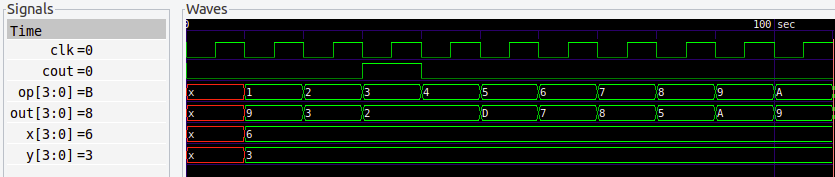
\includegraphics[width=1.05\textwidth]{alu_waveform}
	\caption{ALU Circuit Waveform}
	\label{fig: alu_waveform}
\end{figure}

\begin{figure}[h]
	\centering
	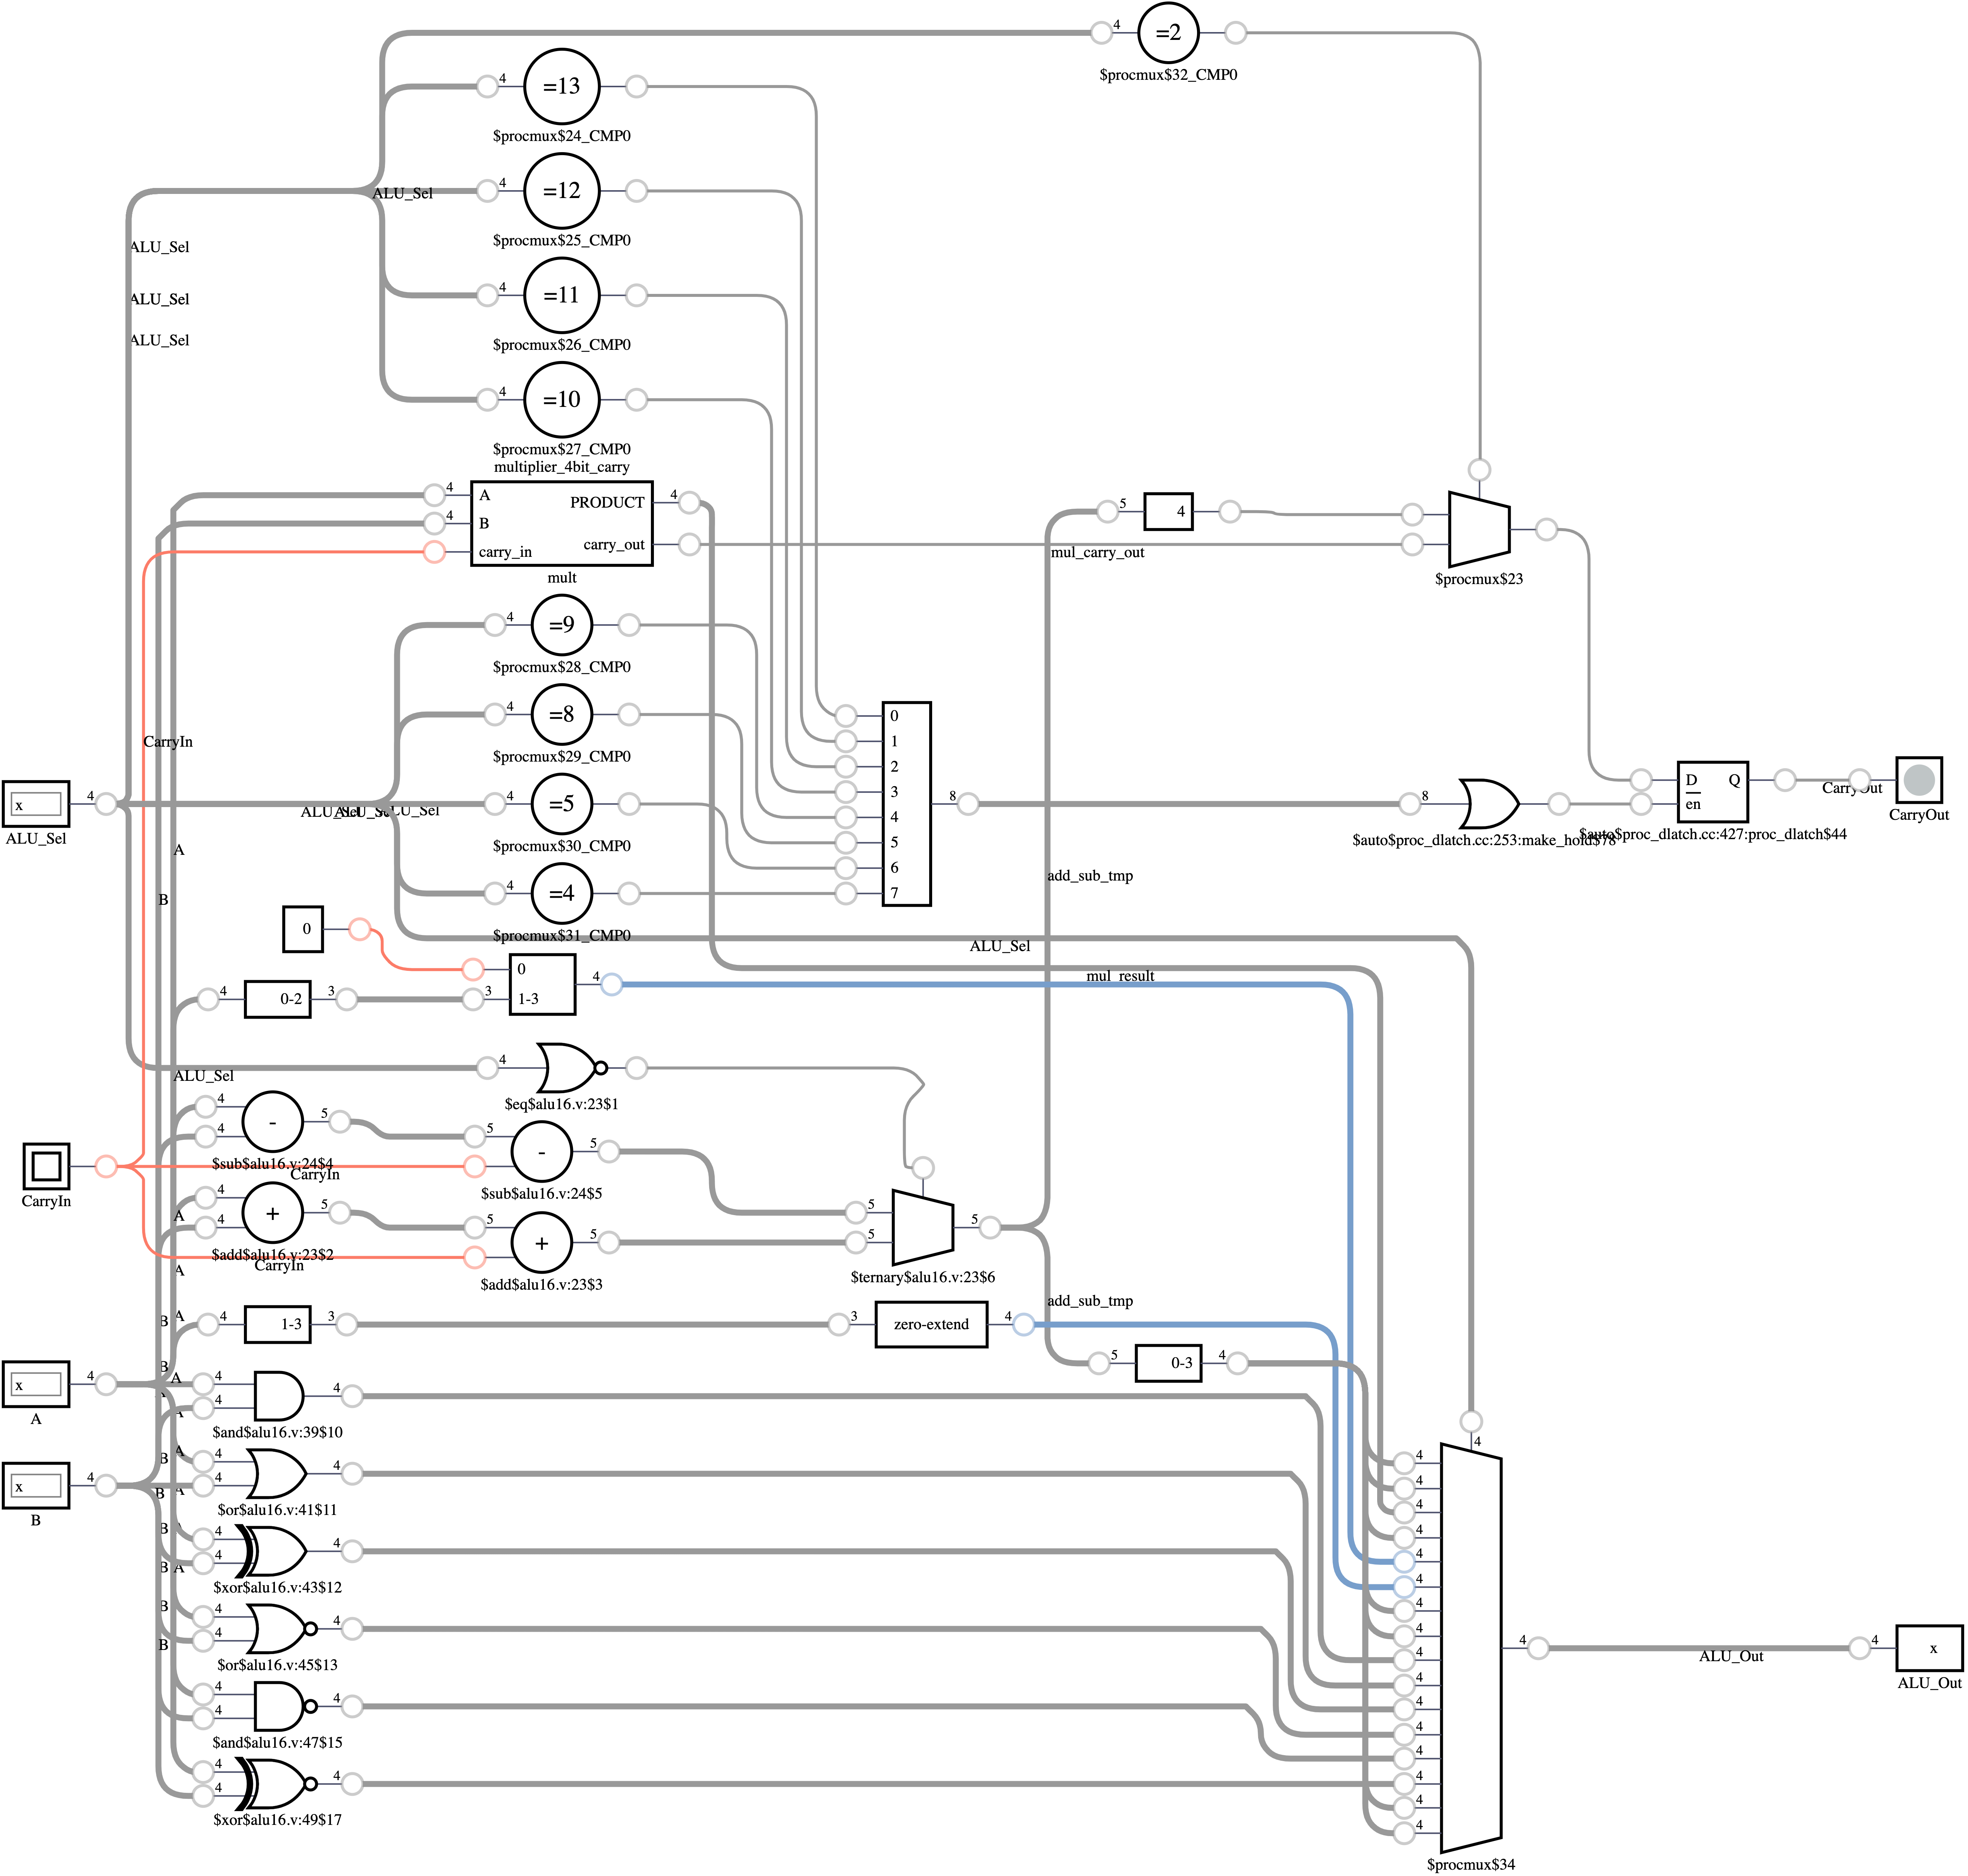
\includegraphics[height=0.67\textheight,width=1.0\textwidth]{alu_circuit}
	\caption{ALU Circuit Diagram}
	\label{fig: alu_circuit}
\end{figure}
\pagebreak

\section{Conclusion}

	Given the requirements for this final project status report, I believe our group got the correct results. The code, test, benches, and waveforms for the 4-bit Binary and 4-bit Arithmetic circuits seems to follow the truth tables and outputs for their corresponding logical and arithmetic operations and inputs, so it seems reasonable that they are correct and our project is successful. The main difficulty our group really ran into was in integrating all the modules together at the same time and choosing only one output based on an opcode received. To fix this problem we called all of the modules and each one had a dedicated output wire (wires r1-r11). All those wires carrying each unique output were fed into the case function acting as a mux and the correct statements were executed based on the opcode the case function/mux received. We did not run into too many obstacles otherwise, as we did not have to set up our virtual environments or do much troubleshooting with the tools we are using, such as Verilog or GTK Wave, and we were able to fairly split up the workload between the three of us quickly and fairly. Once the ALU and its operations were coded and compiled in Verliog, generating the waveforms in GTK Wave and creating the circuit diagrams was fairly straightforward, and all that was left was to gather all the data we created and write the report according to the project requirements.  


 
	
\end{document}
	